\chapter{Background}

% The background section of the report should set the project into context by relating it to existing published work which you read at the start of the project when your approach and methods were being considered. There are usually many ways of solving a given problem, and you shouldn't just pick one at random. Describe and evaluate as many alternative approaches as possible. The published work may be in the form of research papers found in the academic literature, articles, text books, technical manuals, or even existing software or hardware of which you have had hands-on experience. Your must acknowledge the sources of your inspiration. You are expected to have seen and thought about other people's ideas; your contribution will be putting them into practice in some other context. However, avoid plagiarism: if you take another person's work as your own and do not cite your sources of information/inspiration you are being dishonest. When referring to other pieces of work, cite the sources where they are referred to or used, rather than just listing them at the end. Accidental plagiarism or not knowing how to cite and reference is not a valid reason for plagiarism. Make sure you read and digest the Department's plagiarism document .

% In writing the Background chapter you must demonstrate your ability to analyse, synthesise and apply critical judgement. Analysis is shown by explaining how the proposed solution operates in your own words as well as its benefits and consequences. Synthesis is shown through the organisation of your Related Work section and through identifying and generalising common aspects across different solutions. Critical judgement is shown by discussing the limitations of the solutions proposed both in terms of their disadvantages and limits of applicability.

In this chapter, we provide the necessary preliminaries and research context to understand the problem space and proposed solution.

\section{Diabetic Retinopathy} \label{background:classifyingdr}

Diabetic retinopathy is damage to the blood vessels of the retina caused by high blood sugar levels. The level of damage, and hence the stage of DR, can be determined by identifying and categorising different types of lesions on the patient's retina. A description of a subset of these lesions is given as follows \cite{taylor2012handbook}:

\begin{description}
    \item[Microaneurysms (MA)] \hfill \\ Small red round dots caused by weakness in the vessel's walls.
    \item[Haemorrhages (HE)] \hfill \\ Larger spots on the retina.
    \item[Hard exudates (EX)] \hfill \\ Bright yellow spots caused by the leakage of plasma.
    \item[Soft exudates (SE)] \hfill \\ White spots caused by swelling of nerve fibre.
\end{description}

We use color images, not MRI or OCTs or CT scans. Readily available, not as much specialised equipment, telehealth Examples of each type of lesion are shown in \autoref{fig:lesions}.

\begin{figure}
    \centering
    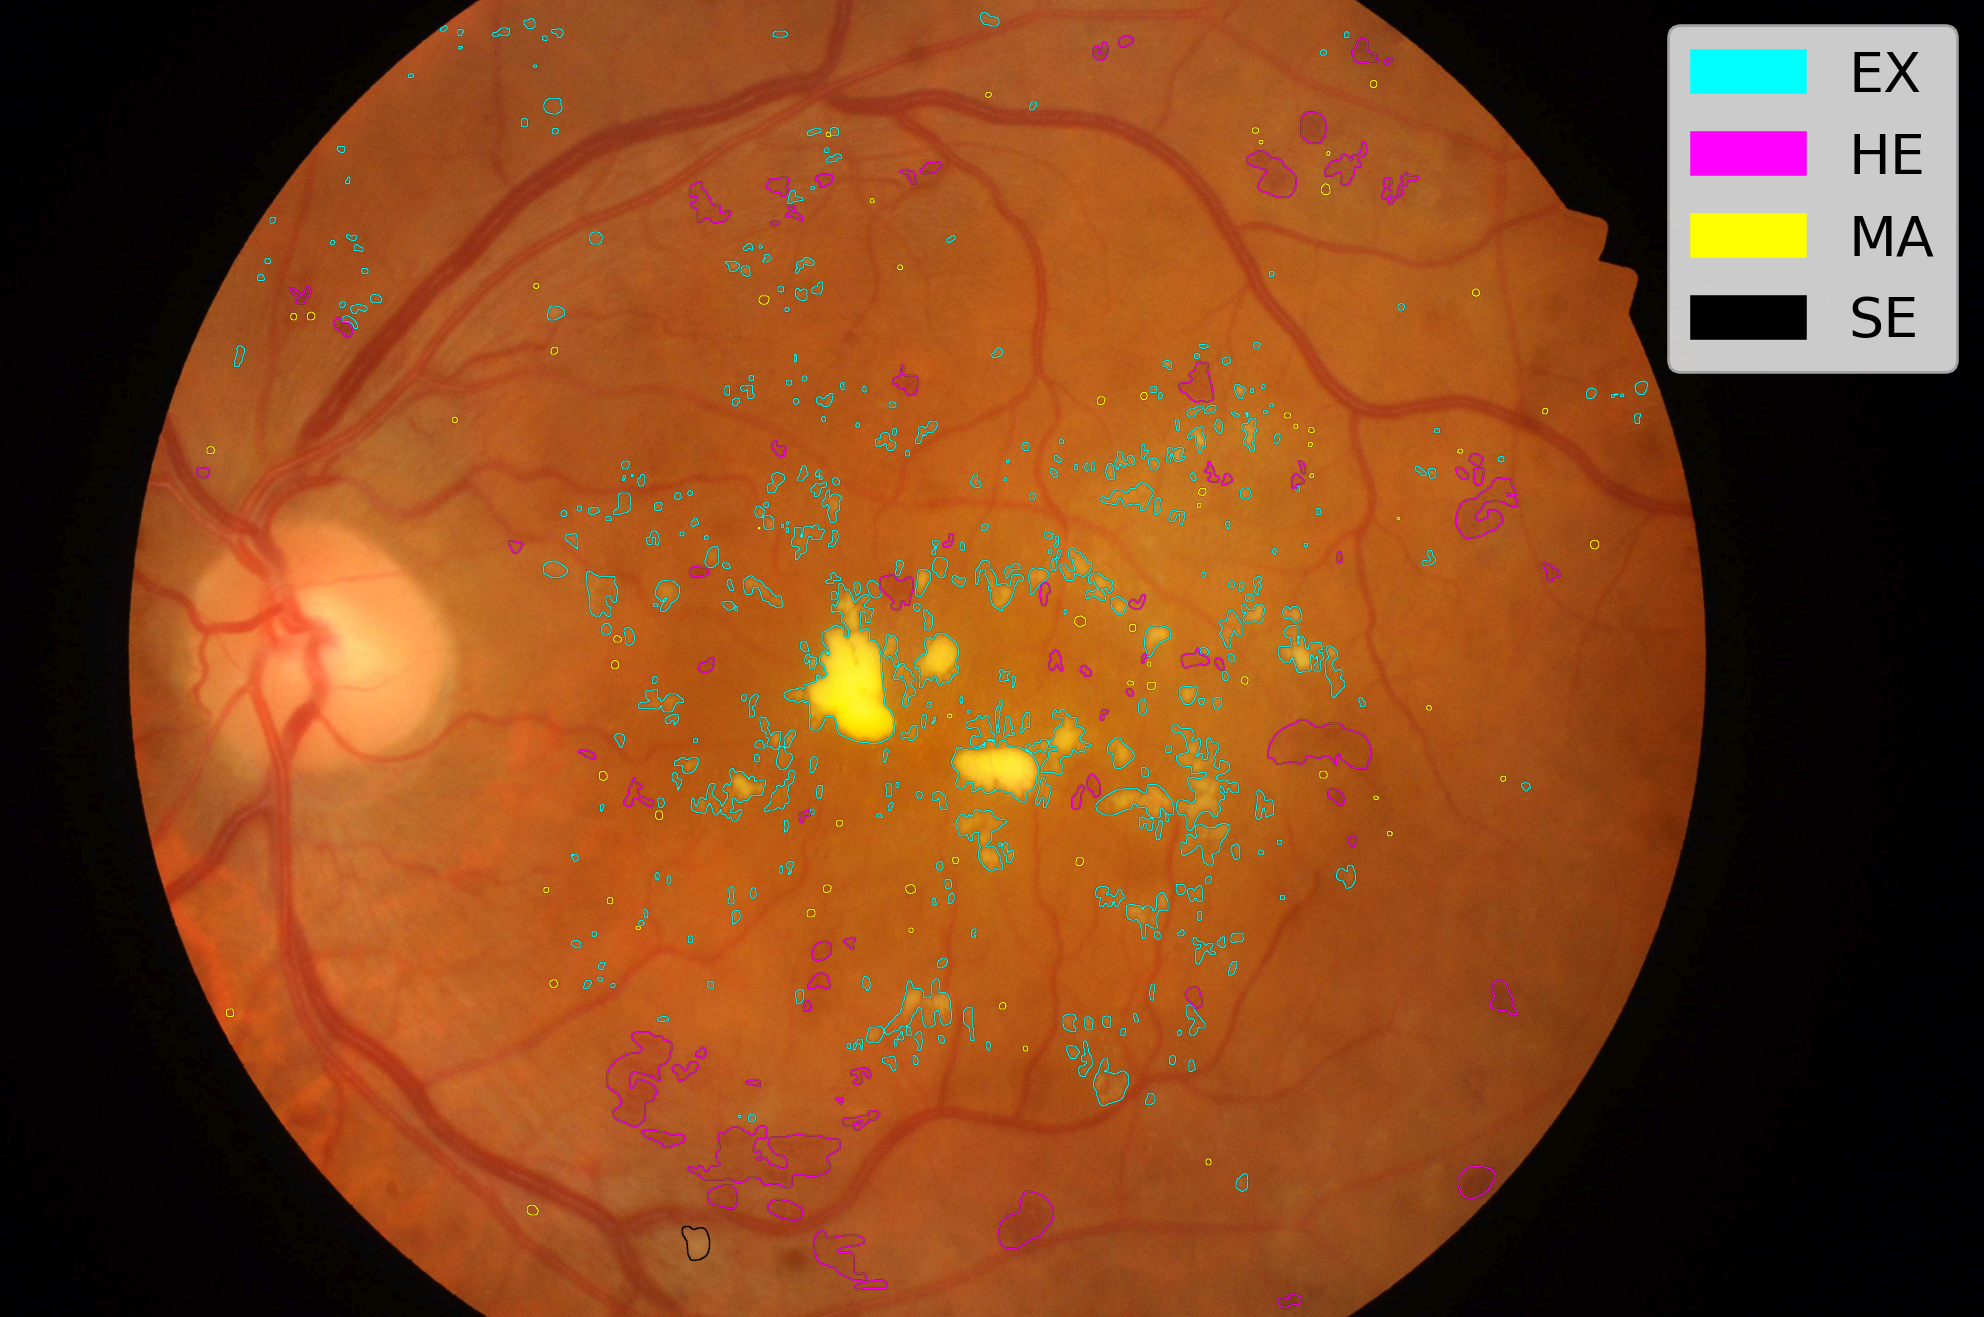
\includegraphics{background/figs/example_output.png}
    \caption{A retinal fundus image annotated with four types of lesions: hard exudates (EX), haemorrhages (HE), microaneurysms (MA), and soft exudates (SE).}
    \label{fig:lesions}
\end{figure}

Clinically, the severity of DR is graded according to an international standard consisting of five stages \cite{ophthalmoscopy2002international}. \autoref{tab:dr_stages} provides a brief summary of the five stages.

\begin{table}
    \centering
    \begin{tabular}{ll}
        \toprule
        Severity & Characteristics \\
        \midrule
        No apparent retinopathy & No abnormalities \\
        Mild NPDR & Microaneurysms only \\
        Moderate NPDR & More than just microaneurysms but less than severe NPDR \\
        Severe NPDR & Any of the following and no signs of PDR: \\ 
        & \tabitem > 20 intraretinal haemorrhages in all 4 quadrants \\
        & \tabitem Venous beading in $\geq$ 2 quadrants\\
        & \tabitem Intraretinal microvascular abnormalities in $\geq$ 1 quadrant \\
        PDR & One or both of: \\
        & \tabitem Neovascularisation \\
        & \tabitem Vitreous/preretinal haemorrhage \\
        \bottomrule
    \end{tabular}
    \caption{The International Clinical Diabetic Retinopathy Disease Scale. \\ NPDR = non-proliferative diabetic retinopathy; PDR = proliferative diabetic retinopathy.}
    \label{tab:dr_stages}
\end{table}

\section{Generative Adversarial Networks}

A Generative Adversarial Network (GAN) is a machine learning framework introduced by Ian Goodfellow in 2014 \cite{NIPS2014_5ca3e9b1} consisting of two neural networks in adversarial competition. The generative model $G$ creates candidate images that look as ``real'' as possible, while the discriminative model $D$ attempts to distinguish between real and synthetic images. Training continues until the discriminator can not longer tell which inputs are fabricated by $G$ and which are real. In this sense, $G$ and $D$ are trained \emph{adversarially}. From this, we can derive the adversarial loss function by taking the cross-entropy of the real and generated functions.
\begin{align} \label{eq:ganloss}
    \mathcal{L}_{GAN} = \mathbb{E}_x[\log D(x)] + \mathbb{E}_z[\log (1-D(G(z))]
\end{align}
where $D(x)$ is the discriminator's estimate that $x$ is real; $G(z)$ is the generator's output when given random noise $z$; $D(G(z))$ is the discriminator's estimate that a fake instance is real. The discriminator will attempt to maximise this loss, whilst the generator will attempt to minimise it. In practice, this happens in alternating phases, keeping the generator fixed when updating the discriminator and vice versa.

The original GAN design is far from perfect, however. In their original paper, \citeauthor{NIPS2014_5ca3e9b1} describe an issue with the original loss formulation where $G$ fails to gain any traction in the early stages of training, and therefore never even begins to converge. This is due to $D$ being able to easily reject to the output of $G$, which causes the gradients to be extremely small. The proposed solution is to, instead of minimising $\log(1-D(G(z))$, \emph{maximise} $\log D(G(z))$.

In no small part to the problems described above, there has been an explosion of GAN variants since their initial introduction. In the following sections, we examine a select few.

\subsection{Conditional GAN}

One of the earliest extensions to the original design, a Conditional GAN (cGAN) extends the vanilla GAN by conditioning on additional information $y$ \cite{mirza2014conditional} This allows us to direct the generation process. Consequently, the loss function previously defined in \autoref{eq:ganloss} now becomes
\begin{align}
    \mathcal{L}_{cGAN} = \mathbb{E}_x[\log D(x|y)] + \mathbb{E}_z[\log (1-D(G(z|y))]
\end{align}

\subsection{ProgressiveGAN}

% Conditional GANs

%% Problems
% Mode collapse.

\section{Image-to-Image Translation}
%  Simulated and Unsupervised Images through Adversarial Training. (2016) Used by Costa
% Image-to-Image Translation with Conditional Adversarial Networks (2016) Used by Costa

\section{Retinal Image Synthesis}

% Automatic Generation of Synthetic Retinal Fundus Images (Fiorini 2014)
% Towards Adversarial Retinal Image Synthesis (Costa 2017)
% Adversarial Synthesis of Retinal Images from Vessel Trees
% End-to-End Adversarial Retinal Image Synthesis (Costa 2017)
% Unsupervised histopathology image synthesis (2017)
% Synthesizing retinal and neuronal images with generative adversarial nets (Tub-GAN) (2018)
% Retinal image synthesis from multiple-landmarks input with generative adversarial networks (2019)
% DR GAN (2020)

Early work surrounding the generation of synthetic retinal fundus images involved patch-based techniques and creating complex mathematical models representing the anatomy of the eye \cite{BONALDI201654, N20103:2014}. Different algorithms had to be proposed for different components of the eye, and computationally expensive operations were used. Heavy use of domain knowledge.

More recently, purely data-driven approaches have been shown to be highly effective. In 2017, \citeauthor{DBLP:journals/corr/CostaGMANMC17} published their foundational work utilising GANs for retinal image synthesis \cite{DBLP:journals/corr/CostaGMANMC17}. The proposed generator network operated by performing image-to-image translation from a vessel network to a retina image. They borrow from CITE, CITE, mentioned above by implementing an adversarial loss function that not only . 

In the absence of a large dataset containing manual annotations, vessel segmentation masks were inferred from the output of a segmentation model. Hence, from a single vessel network, an unbounded number of complete retinal fundus images sharing the same vascular structure could be obtained. However, this approach still suffered some major drawbacks. The generator relies on a vessel segmentation mask as input. This is unideal since the user will have to either (a) manually obtain their own vessel segmentation, which in and of itself is a lot of work, (b) use a pre-existing vessel segmentation, which there is a limited pool of, or (c) infer a vessel segmentation (as the authors did) which may be unreliable. It's worth noting that a poorly inferred vessel network, as may be produced by a segmentation model, fails to produce a usable fundus image as pointed out by the paper's authors. Moreover, the output images have a resolution of $512 \times 512$ which, while large relative to the images often used in computer vision publications, is small compared to those produced by modern fundus photography.

The same authors continued to refine these techniques in a later work \cite{8055572}. The major extension offered by this paper was removing the dependency on a pre-existing vessel segmentation as input. Instead, an adversarial autoencoder is employed to generate vessels segmentation masks, which can be fed into the previously described image-to-image model, requiring the user to simply supply a sample from a multivariate normal distribution. While this overcomes the first of the issues with the previous work by obviating the need to obtain a segmentation mask, the issue of resolution remains. Furthermore, it is noted that the autoencoder does not always generate anatomically correct vascular structures.

\citeauthor{ZHAO201814} incrementally built upon this work in 2018 by introducing Tub-GAN. It is similar to its predecessor in that the same adversarial loss function is sued. The notable improvements are the fact that manual annotations are used. Different outputs from the same input. 

They both use the same loss-function. Both use basic generator architecture but slightly modified. Tub-GAN uses tanh instead of sigmoid.

A few shortcomings are noted. First, the optic disc is blurred.

While representing an important step towards the generation of synthetic fundus images, these methods do not have any relation to DR i.e. generating pathological instances.

DR-GAN uses more recent developments in machine learning like multi-spatial attention.